\chapter{Introduction}
\label{cha:Introduction} % Ein Label ist optional, ermoeglicht aber die Referenzierung
Situation nowadays -> Lots of data (industry 4.0, other use cases, etc.)

Motivation
Goal -> Research question definieren und spezifizieren, discuss the different architectures
Struktur erläutern

% Introduction: lots of data -> cant save it all -> need a way to deal with it
% Examples of when it is applied
% How does it work, are there alternatives? yes -> batch processing (Maybe briefly explain)
The advancements in technology of the past decades has lead to enormous data creation. Technology has become ubiquitous, 
with the evolution of cell phones to smartphones, the digitilization of industrial processes, Industry 4.0
and the increasing amount of ``smart`` devices, causing creation of information to grow exponentially.
It is estimated that the \gls{datasphere} will reach the size of 175 zettabytes by 2025, as shown in figure 1.1.
% Graph estimating the growth of the global datasphere (by IDC)
\begin{figure}[ht]
\centering
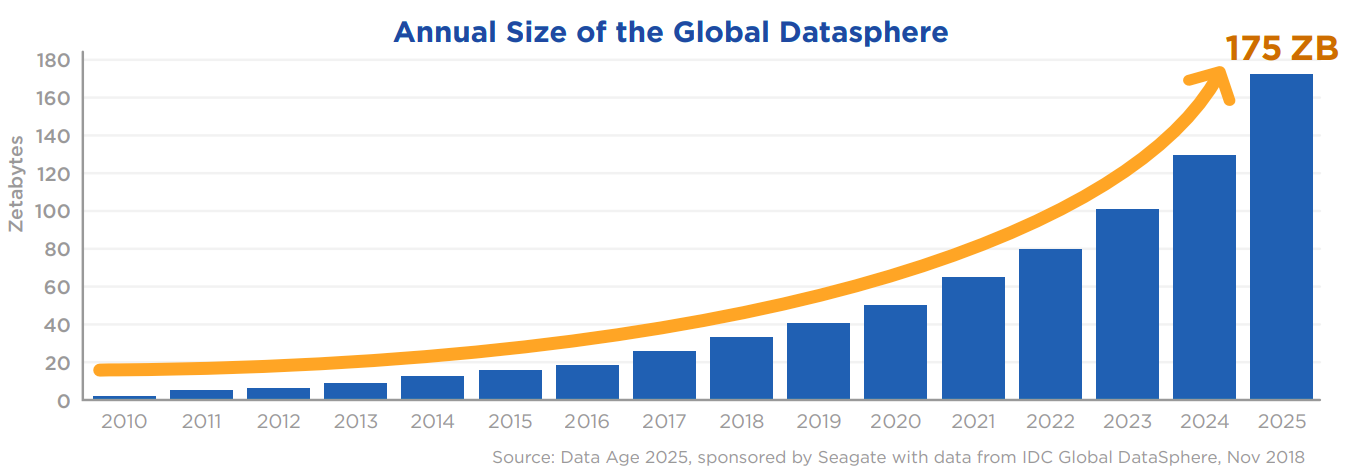
\includegraphics[width=1.0\textwidth]{Bilder/size_global_datasphere.png}
\caption{The Growth of the Global Datasphere \cite[p.6]{idc-seagate-data}}
\label{fig:growth_datasphere}
\end{figure}

% Maybe a source here?
Data has become an important factor in decision making and optimization in virtually every industry, especially in finances. \fett{TODO: Wieso?}
The financial market is dominated by data driven decisions, with emphasis on data processing in a (near) real-time fashion.
However, real-time data is becoming of importance in multiple sectors; the International Data Corporation estimates that real-time data will be 
responsible for a share of 30 percent of the total global datasphere by 2025, as shown in figure 1.2.
% Graph showing the growing share of real-time data as part of global datasphere
\begin{figure}[h]
\centering
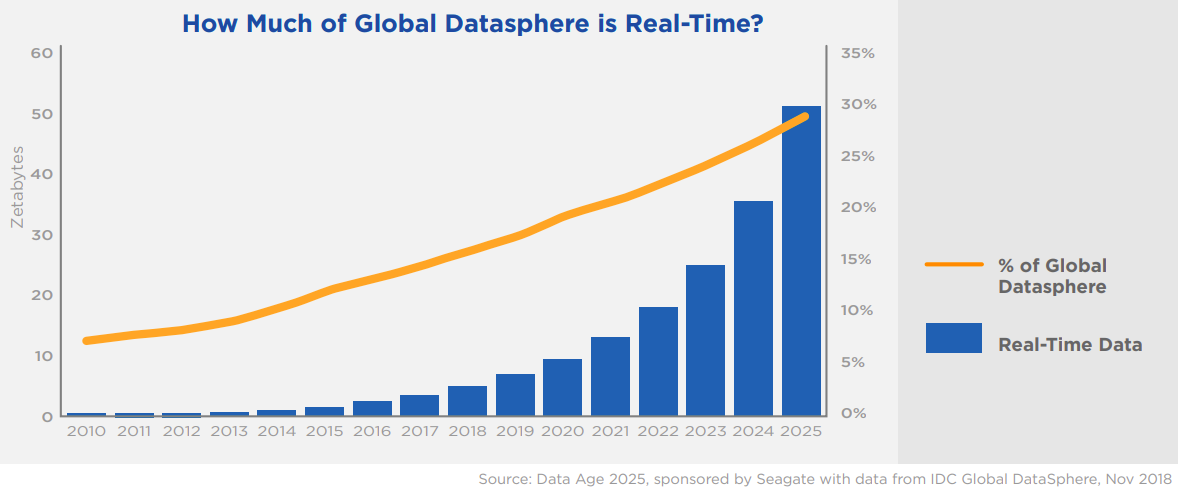
\includegraphics[width=1.0\textwidth]{Bilder/realtime_data.png}
\caption{The growth of real-time data as part of the Global Datasphere \cite[p.13]{idc-seagate-data}}
\label{fig:growth_realtime_data}
\end{figure}

A global study led by IBM in 2012 has shown that 71 percent of the firms in the financial market use information (including big data)
in order to achieve an advantage over their competitors, compared to 36 percent, which IBM has found in an earlier study conducted in 2010. \cite[p.1]{ibm-financial}

As it is no longer feasible to save all the data before then analyzing it (in batches), due to computational cost and lack of storage capacity, 
a new approach was designed in order to handle data in a (near) real-time fashion, Stream Processing Systems (SPS).
\fett{TODO: SPS Traditional DBMS.. another reason and then dsms}
